% ============================================================
\chapter{R\'esolution Num\'erique des EDO}
\label{ch:edo}
% ============================================================

\section{Exemple motivant}
Le mouvement d'un pendule simple est r\'egi par $\theta''=-\frac{g}{L}\sin\theta$. Pour de grandes oscillations, pas de solution analytique. On discr\'etise en temps et on it\`ere.

\section{Probl\`eme de Cauchy}

\begin{definition}
\[
y'(t) = f(t,y(t)), \quad y(t_0)=y_0, \quad t\in[t_0,T].
\]
Discr\'etisation : $t_n=t_0+nh$, $y_n\approx y(t_n)$.
\end{definition}

\section{M\'ethode d'Euler explicite}\index{Euler!explicite}

\begin{definition}
\[
y_{n+1} = y_n + h\,f(t_n,y_n).
\]
\end{definition}

\begin{algorithm}[H]
\caption{Euler explicite}\label{alg:euler}
\KwEntree{$f$, $t_0$, $T$, $y_0$, $h$}
\KwSortie{$(t_n,y_n)_{n=0}^N$}
$N\gets\lfloor(T-t_0)/h\rfloor$\;
\Pour{$n=0,\ldots,N-1$}{
  $y_{n+1}\gets y_n+h\,f(t_n,y_n)$\;
  $t_{n+1}\gets t_n+h$\;
}
\end{algorithm}

\begin{theoreme}[Erreur locale et globale d'Euler]
\begin{itemize}
\item Erreur locale de troncature : $\tau_n=\frac{y(t_{n+1})-y(t_n)}{h}-f(t_n,y(t_n))=\BigO(h)$.
\item Erreur globale : $\max_n|y(t_n)-y_n|=\BigO(h)$ (m\'ethode d'ordre 1).
\end{itemize}
\end{theoreme}

\begin{proof}[Esquisse]
Par Taylor : $y(t_{n+1})=y(t_n)+hy'(t_n)+\frac{h^2}{2}y''(\xi)$. Donc $\tau_n=\frac{h}{2}y''(\xi)=\BigO(h)$. L'erreur globale s'accumule sur $N=T/h$ pas : $e_N\leq\frac{e^{LT}-1}{L}\cdot\max|\tau_n|=\BigO(h)$.
\end{proof}

\section{M\'ethode d'Euler implicite}\index{Euler!implicite}

\begin{definition}
\[
y_{n+1} = y_n + h\,f(t_{n+1},y_{n+1}).
\]
N\'ecessite la r\'esolution d'une \'equation (Newton) \`a chaque pas. Avantage : \textbf{A-stabilit\'e}.
\end{definition}

\section{M\'ethodes de Runge--Kutta}\index{Runge--Kutta}

\begin{definition}[RK4 classique]
\begin{align}
k_1 &= f(t_n,y_n), \\
k_2 &= f(t_n+h/2,\; y_n+hk_1/2), \\
k_3 &= f(t_n+h/2,\; y_n+hk_2/2), \\
k_4 &= f(t_n+h,\; y_n+hk_3), \\
y_{n+1} &= y_n + \frac{h}{6}(k_1+2k_2+2k_3+k_4).
\end{align}
\end{definition}

\begin{theoreme}[Ordre de RK4]
RK4 est d'ordre 4 : erreur globale $\BigO(h^4)$.
\end{theoreme}

\section{Tableau de Butcher}

\begin{definition}
Un sch\'ema de Runge--Kutta \`a $s$ \'etages est d\'efini par :
\[
\begin{array}{c|c}
\mathbf{c} & A \\
\hline
& \mathbf{b}^\top
\end{array}
\]
Pour RK4 :
$\begin{array}{c|cccc}
0 & & & & \\
1/2 & 1/2 & & & \\
1/2 & 0 & 1/2 & & \\
1 & 0 & 0 & 1 & \\
\hline
& 1/6 & 1/3 & 1/3 & 1/6
\end{array}$
\end{definition}

\section{Stabilit\'e}\index{A-stabilite@A-stabilit\'e}

\begin{definition}[\'Equation test]
$y'=\lambda y$, $\lambda\in\C$, $\text{Re}(\lambda)<0$. Le facteur d'amplification est $R(z)$ avec $z=h\lambda$ : $y_{n+1}=R(z)y_n$.
\begin{itemize}
\item Euler explicite : $R(z)=1+z$. Stable si $|1+z|<1$.
\item Euler implicite : $R(z)=1/(1-z)$. Stable pour tout $\text{Re}(z)<0$ (A-stable).
\item RK4 : $R(z)=1+z+z^2/2+z^3/6+z^4/24$.
\end{itemize}
\end{definition}

\begin{center}
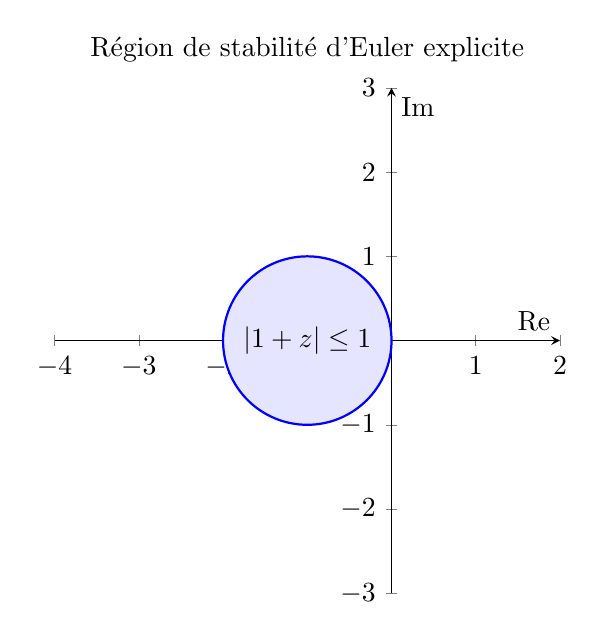
\begin{tikzpicture}
\begin{axis}[
  width=8cm, height=8cm, axis equal, axis lines=middle,
  xlabel={Re}, ylabel={Im}, xmin=-3.5, xmax=1.5, ymin=-3, ymax=3,
  title={R\'egion de stabilit\'e d'Euler explicite}
]
\draw[thick,blue,fill=blue!10] (-1,0) circle (1);
\node at (axis cs:-1,0) {$|1+z|\leq 1$};
\end{axis}
\end{tikzpicture}
\end{center}

\section{Exemple num\'erique}

$y'=-y$, $y(0)=1$, solution exacte $y=e^{-t}$.

\begin{center}
\begin{tabular}{ccccc}
\toprule
$h$ & Euler & Err. Euler & RK4 & Err. RK4 \\
\midrule
0.1 & 0.348678 & $1{,}9\times10^{-2}$ & 0.367879 & $3{,}8\times10^{-8}$ \\
0.05 & 0.358486 & $9{,}4\times10^{-3}$ & 0.367879 & $2{,}4\times10^{-9}$ \\
0.01 & 0.366032 & $1{,}8\times10^{-3}$ & 0.367879 & $<10^{-15}$ \\
\bottomrule
\end{tabular}
\end{center}

\section{Impl\'ementation}

\begin{codeblock}[title=\textbf{Python}]
\begin{minted}{python}
import numpy as np
import matplotlib.pyplot as plt

def euler(f, t0, T, y0, h):
    t = np.arange(t0, T+h, h)
    y = np.zeros((len(t), len(np.atleast_1d(y0))))
    y[0] = y0
    for n in range(len(t)-1):
        y[n+1] = y[n] + h * np.array(f(t[n], y[n]))
    return t, y

def rk4(f, t0, T, y0, h):
    t = np.arange(t0, T+h, h)
    y = np.zeros((len(t), len(np.atleast_1d(y0))))
    y[0] = y0
    for n in range(len(t)-1):
        k1 = np.array(f(t[n], y[n]))
        k2 = np.array(f(t[n]+h/2, y[n]+h*k1/2))
        k3 = np.array(f(t[n]+h/2, y[n]+h*k2/2))
        k4 = np.array(f(t[n]+h, y[n]+h*k3))
        y[n+1] = y[n] + h/6 * (k1 + 2*k2 + 2*k3 + k4)
    return t, y

# Test : y' = -y
f = lambda t, y: -y
t_e, y_e = euler(f, 0, 1, [1.0], 0.1)
t_r, y_r = rk4(f, 0, 1, [1.0], 0.1)
exact = np.exp(-t_e)

plt.figure(figsize=(8, 5))
plt.plot(t_e, exact, 'k-', lw=2, label='Exact')
plt.plot(t_e, y_e, 'ro--', label='Euler')
plt.plot(t_r, y_r, 'bs-', label='RK4')
plt.legend(); plt.xlabel('t'); plt.ylabel('y')
plt.title("Euler vs RK4"); plt.savefig("ch09_edo.pdf"); plt.show()
\end{minted}
\end{codeblock}

\begin{codeblock}[title=\textbf{Julia}]
\begin{minted}{julia}
function rk4(f, t0, T, y0, h)
    t = t0:h:T
    y = [copy(y0)]
    for n in 1:length(t)-1
        yn = y[end]
        k1 = f(t[n], yn)
        k2 = f(t[n]+h/2, yn .+ h/2 .* k1)
        k3 = f(t[n]+h/2, yn .+ h/2 .* k2)
        k4 = f(t[n]+h, yn .+ h .* k3)
        push!(y, yn .+ h/6 .* (k1 .+ 2k2 .+ 2k3 .+ k4))
    end
    return collect(t), y
end

f(t, y) = -y
t, y = rk4(f, 0.0, 1.0, [1.0], 0.1)
println("y(1) = $(y[end][1]), exact = $(exp(-1))")
\end{minted}
\end{codeblock}

\section{Exercices}

\begin{exercice}[$\star$]
Appliquer Euler explicite \`a $y'=y$, $y(0)=1$, $h=0{,}1$, pour $t\in[0,1]$. Comparer \`a $e^t$.
\end{exercice}

\begin{exercice}[$\star\star$]
Montrer que RK4 est d'ordre 4 en d\'eveloppant $y(t+h)$ par Taylor jusqu'au terme $h^4$.
\end{exercice}

\begin{exercice}[$\star\star$]
Tracer la r\'egion de stabilit\'e de RK4 num\'eriquement.
\end{exercice}

\begin{exercice}[$\star\star\star$ -- Projet]
R\'esoudre le syst\`eme de Lorenz $(\sigma=10,\rho=28,\beta=8/3)$ par RK4. Visualiser l'attracteur en 3D. \'Etudier la sensibilit\'e aux conditions initiales.
\end{exercice}

\begin{formules}
\begin{align*}
\text{Euler} &: y_{n+1}=y_n+hf(t_n,y_n), \quad \BigO(h) \\
\text{RK4} &: y_{n+1}=y_n+\tfrac{h}{6}(k_1+2k_2+2k_3+k_4), \quad \BigO(h^4) \\
\text{Stabilit\'e} &: |R(h\lambda)|<1
\end{align*}
\end{formules}
